\section{Communication with openHAB}
\label{sec:design:communication-with-openhab}

The open source home automation hub openHAB described in \Cref{sec:analysis:choice-of-hub} exposes an API with a REST architecture. Clients can communicate with the API over HTTP.

The communication with the openHAB API consists of the following two components.

\begin{description}
\item[REST client] A base REST client suitable for communicating with a REST API which carries its data using JSON. The client implements base methods for interacting with a REST API. This includes retrieving, deleting, updating and creating entities. The base client parses data received by the API into models.
\item[openHAB client] The client builds on top of the base REST client and adds openHAB specific methods. This includes retrieving things and items as well as updating the state of an item.
\end{description}

\Cref{fig:design:communication-with-openhab:class-diagram-rest-client} shows a class diagram of the REST client. The involved components are briefly described below.

\begin{description}
\item[RESTClient] The base REST client which is responsible for performing requests and mapping response to models that can be further processed or displayed in the application.
\item[RequestQueue] Responsible for creating worker threads for network requests.
\item[ResultListener] Interface implemented by objects that should receive a result when a network request completes, either because of a failure or because of a succesful response.
\item[EntityBuilder] Interface implemented by objects mapping from the received JSON to models.
\item[Result] Encapsulates a network result. A result can either be a success or a failure. In case of a success, the result will contain a the value received from the API. In case of a failure, the result must contain an error.
\end{description}

\begin{figure}[h!]
\centering
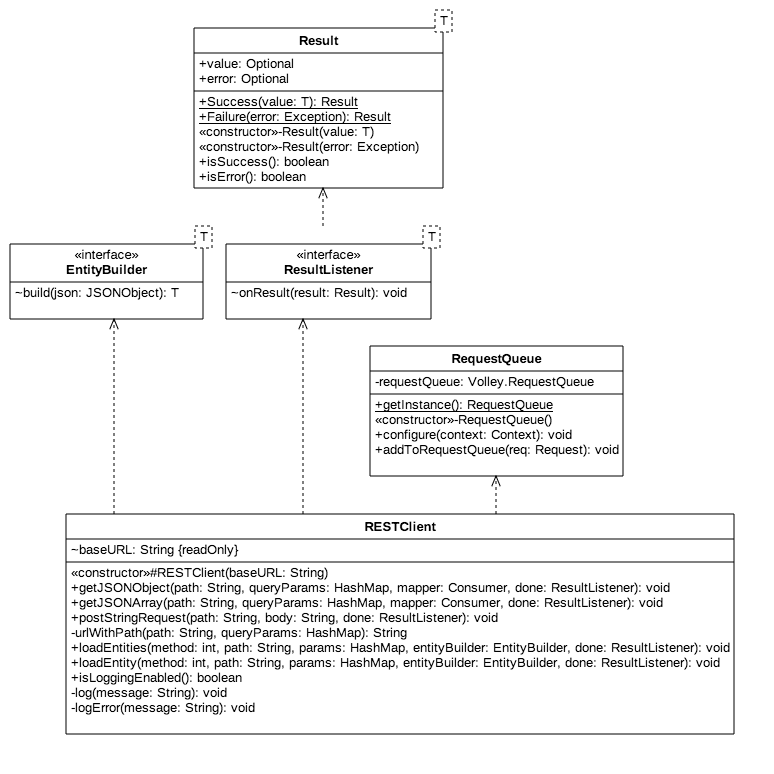
\includegraphics[width=\textwidth]{images/uml-rest-client}
\caption{Class diagram showing the architecture of the REST client used for communicating with a REST API.}
\label{fig:design:communication-with-openhab:class-diagram-rest-client}
\end{figure}

\Cref{fig:design:communication-with-openhab:class-diagram-openhab-client} shows a class diagram of the openHAB client. The involved components are briefly described below.

\begin{description}
\item[OpenHABClient] A specialization of the base REST client implementing openHAB specific functionality.
\item[BooleanResult] Similar to the Result, this either represents a success or a failure. In the case of a success, the BooleanResult does not contain a value.
\item[Item] Model representing an item in openHAB.
\item[Thing] Model representing a thing in openHAB.
\end{description}

\begin{figure}[h!]
\centering
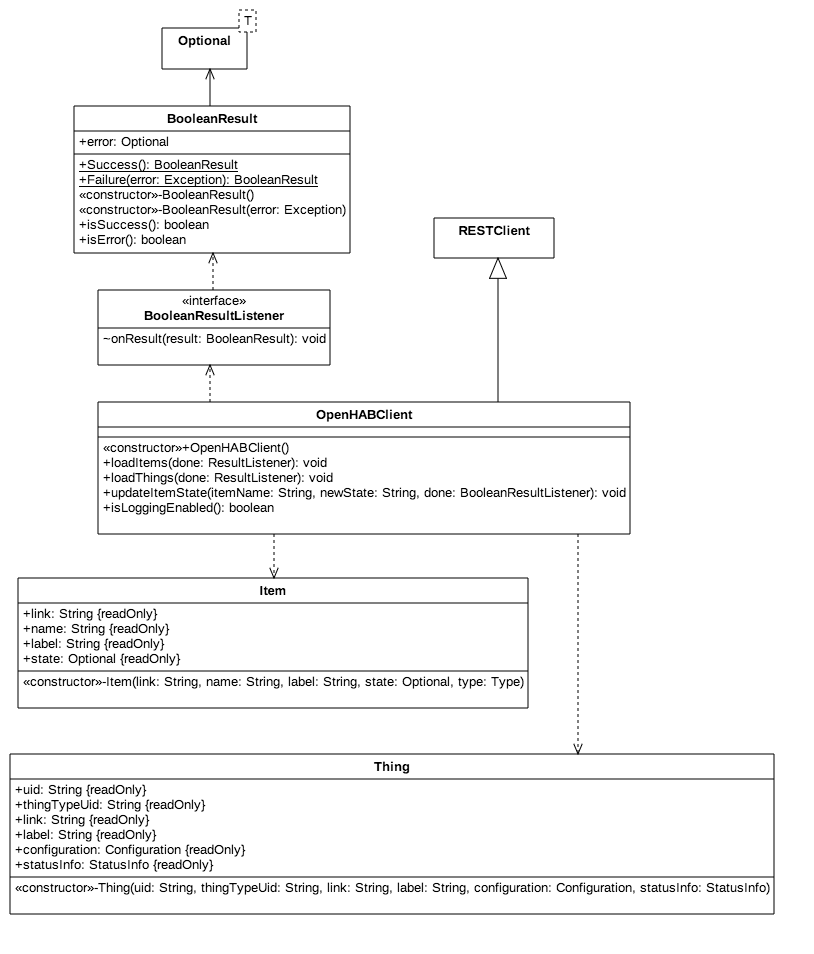
\includegraphics[width=\textwidth]{images/uml-openhab-client}
\caption{Class diagram showing the architecture of the openHAB client used for communicating with the openHAB API}
\label{fig:design:communication-with-openhab:class-diagram-openhab-client}
\end{figure}

\subsection{Mapping of Actions}

Eclipse SmartHome, which openHAB builds on top of, has a set of supported item types. An item type defines which actions an item supports. \Cref{tbl:design:communication-with-openhab:types} shows a list of the item types supported by Eclipse SmartHome and thus also by openHAB. For each item type, the actions supported by the item type is listed. Item types DateTime and Group are special items in openHAB which has no support for actions but is used to hold a date and time and a group of other items respectively.
The action types ``Percent'', ``HSB'', ``Decimal'' and ``String'' are not exact actions that can be send to openAB but refers to type of action, e.g. a lamp supporting the ``Percent'' action can receive a request containing ``50'' and adjust its brightness to 50\%. The other action types are exat actions that can be send in a request to openHAB.

In the smartwatch application, we create a list of supported actions for each item. A supported action for an item is represented as the string, which is sent to openHABs API when an action should be triggered. For example, an item of type Switch has the set of actions $\{ "ON", "OFF" \}$. For the sake of this prototype, we only support a limited subset of item types and actions. The supported types and actions are shown in \Cref{tbl:design:communication-with-openhab:types}.

\begin{table}[]
\centering
\caption{Supported actions for each item type in openHAB \cite{eclipse:smarthomeitems}.}
\label{tbl:design:communication-with-openhab:types}
\begin{tabular}{p{2cm}p{6cm}p{6cm}}
\textbf{Item type} & \textbf{Description}                              & \textbf{Action types}                      \\ 
Color              & Color information (RGB)                           & ON, OFF, INCREASE, DECREASE, Percent, HSB      \\
Contact            & Item storing status of e.g. door/window contacts  & OPEN, CLOSE                                  \\
DateTime           & Stores date and time                              &                                            \\
Dimmer             & Item carrying a percentage value for dimmers      & ON, OFF, INCREASE, DECREASE, Percent           \\
Group              & Item to nest other items / collect them in groups &                                            \\
Number             & Stores values in number format                    & Decimal                                    \\
Player             & Allows to control players (e.g. audio players)    & PLAY, PAUSE, NEXT, PREVIOUS, REWIND, FASTFORWARD \\
Rollershutter      & Typically used for blinds                         & UP, DOWN, STOP, MOVE, Percent                  \\
String             & Stores texts                                      & String                                     \\
Switch             & Typically used for lights (on/off)                & ON, OFF                                     
\end{tabular}
\end{table}

\begin{table}[]
\centering
\caption{Actions supported by the smartwatch application.}
\label{tbl:design:communication-with-openhab:supported-types}
\begin{tabular}{p{2cm}p{11cm}}
\textbf{Item type}      & \textbf{Action types}                      \\ 
Dimmer                  & ON, OFF, INCREASE, DECREASE, 10, 20, 30, 40, 50, 60, 70, 80, 90           \\
Switch                  & ON, OFF                                     
\end{tabular}
\end{table}

%%% Local Variables:
%%% mode: latex
%%% TeX-master: "../../master"
%%% End:
